\documentclass[12pt,a4paper]{article}

\usepackage{a4wide}
\usepackage{csvsimple}
\usepackage{amsmath}
\usepackage{booktabs}
\usepackage{amssymb}
\usepackage{nicefrac}
\usepackage{enumitem}
\usepackage{float}
\usepackage{todonotes}
\usepackage[breaklinks,plainpages=false,pdfpagelabels]{hyperref}
\hypersetup{colorlinks,citecolor=blue,filecolor=blue,linkcolor=blue,urlcolor=blue}
\usepackage{graphicx}
\setlength\parindent{0pt} % no paragraph indents
\setlength\parskip{6pt} % paragraph vertical spacing
\usepackage{circuitikz} % for circuit diagrams
\usepackage{pgfplots}
\usepackage{tikz}
\usetikzlibrary{positioning,shapes,shadows,arrows,calc}
\DeclareMathOperator{\sinc}{sinc} %sinc
\usepackage[normalem]{ulem} %strike out text using \sout

\usepackage{fancyhdr}
\pagestyle{fancy}
\fancyhead[L]{CSSE4010: Digital Doo-Hickeys}
\fancyhead[R]{Sem 2, 2023}


%---------------------------------------------------------------%
%                                                               %
%               environment definitions                         %
%                                                               %
%---------------------------------------------------------------%
\newcounter{boldalphcounter}
\renewcommand{\theboldalphcounter}{(\alph{boldalphcounter})}
\newenvironment{boldalphlist}{\begin{list}{\textbf{\theboldalphcounter}}%
  {\usecounter{boldalphcounter}}}{\end{list}}

\newcounter{alphcounter}
\renewcommand{\thealphcounter}{(\alph{alphcounter})}
\newenvironment{alphlist}{\begin{list}{\thealphcounter}%
  {\usecounter{alphcounter}}}{\end{list}}

\newcounter{romancounter}
\renewcommand{\theromancounter}{\roman{romancounter})}
\newenvironment{romanlist}{\begin{list}{\textbf{\theromancounter}}%
  {\usecounter{romancounter}}}{\end{list}}

\newcounter{boldarabiccounter}
\renewcommand{\theboldarabiccounter}{\arabic{boldarabiccounter}}
\newenvironment{boldarabiclist}{\begin{list}{\textbf{\theboldarabiccounter.}}%
  {\usecounter{boldarabiccounter}}}{\end{list}}

 % Counter
\newcounter{questioncounter}

\begin{document}

\begin{center}
\bigskip
\section*{CSSE4010 A1}
\end{center}

David Gaul

s4671313

Lab Session: Wednesday 10-12

Submission Date: 7th August

\section{Introduction}

There were two main goals to the first practical. The first of these goals was to familiarise the students with the CSSE4010 work environment. Students were required to download Vivado and install the necessary cable drivers. Basic introductory programs were then taught to the student so that they could familiarise themselves with the unique VHDL syntax.

Which is a pretty good syntax. Very Python-y.

The second task, on which this report is based, was to develop a self-checking test bed to automatically and exhaustively check the functionality of the AND2OR design: a simple connection of two AND gates connecting to an OR gate (Diagram schematics will be provided within the design description). Test cases had to be developed in three separate forms: structural, behavioural and flow, and tested individually. Lastly, propagation delay had to be integrated into the simulation to emulate the delays that would be experienced in real life due to wires and computing time.

This report will detail the design process for developing this test bed. It will include a design description, where the methodology is explained, results of the successful simulation, synthesis and implementation before a final discussion of results and conclusion. 

Let's get cracking.

\section{Design Description}

As detailed within the introduction, a test bed had to be created to check the functionality of the AND2OR program. This featured a series combination of two AND gates connecting to an output OR gate. The block diagram representation of this can be found in fig. \ref{fig:cct}

\begin{figure}[H]
    \centering
    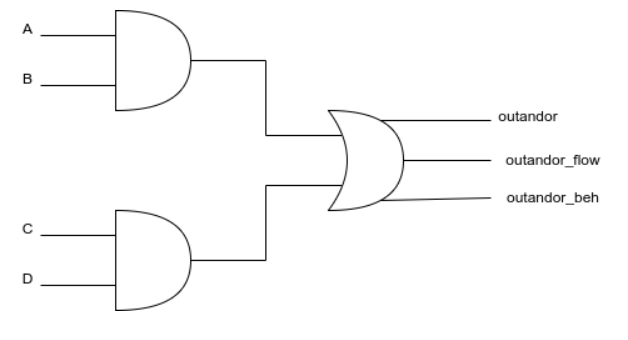
\includegraphics[scale=0.5]{images/cct.png}
    \caption{Circuit representation of AND2OR}
    \label{fig:cct}
\end{figure}

As can be seen, this model requires the following I/O:

\begin{itemize}
  \item 4 inputs - a, b, c, d
  \item 3 outputs - outandor, $outandor \_ flow$ and $outandor \_ beh$
\end{itemize}

Where all three outputs are identical, except they are expressed in structural, flow and behavioural syntax respectively. This can be represented in terms of boolean algebra as:

\[F = (a \cap b) \cup (c \cap d)\]

Hopefully I got the $\cap$ and $\cup$ the right way around. I always get them mixed up $-.-$

Anyway

The truth table of this system, which will form the basis of the test bed design, can be found within table \ref{tab:truth_table}

\begin{table}[H]
\centering
\begin{tabular}{lllll}
A & B & C & D & F \\
0 & 0 & 0 & 0 & 0 \\
0 & 0 & 0 & 1 & 0 \\
0 & 0 & 1 & 0 & 0 \\
0 & 0 & 1 & 1 & 1 \\
0 & 1 & 0 & 0 & 0 \\
0 & 1 & 0 & 1 & 0 \\
0 & 1 & 1 & 0 & 0 \\
0 & 1 & 1 & 1 & 1 \\
1 & 0 & 0 & 0 & 0 \\
1 & 0 & 0 & 1 & 0 \\
1 & 0 & 1 & 0 & 0 \\
1 & 0 & 1 & 1 & 1 \\
1 & 1 & 0 & 0 & 1 \\
1 & 1 & 0 & 1 & 1 \\
1 & 1 & 1 & 0 & 1 \\
1 & 1 & 1 & 1 & 1
\end{tabular}
\caption{Truth table for AND2OR program}
\label{tab:truth_table}
\end{table}

The structural schematic was further verified through the RTL diagram shown in figure \ref{fig:rtl}. As a side note, it can be seen that Vivado's optimisation combined the flow and behavioural models, thus giving them the same output.

\begin{figure}[H]
    \centering
    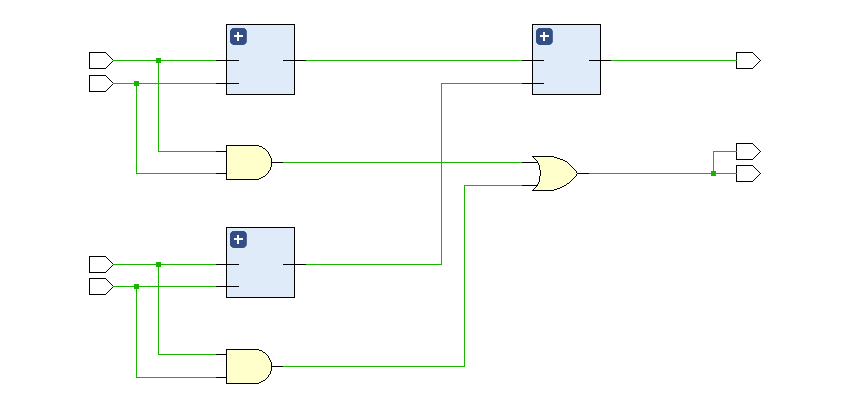
\includegraphics[scale=0.5]{images/rtl.png}
    \caption{RTL representation of AND2OR}
    \label{fig:rtl}
\end{figure}

Didn't label inputs and outputs here. We can safely say that we get the idea.

It's worth noting here that this section does not go into great detail into the design methodology of the circuit. That's because we were provided with the file containing two AND gates connecting to an OR gate. No designing required. Even a monkey like me can work with that.

\section{Simulation Results}

In creating the test bed, it was important to iterate over each of the possible input combinations, and test the outputs for each of the structural, behavioural and flow models. This iteration was achieved using a for loop. Code for this can be found within the appendices. In stress testing the system for every possible input, the following outputs were attained in figure \ref{fig:simulation_no_delay}

\begin{figure}[H]
    \centering
    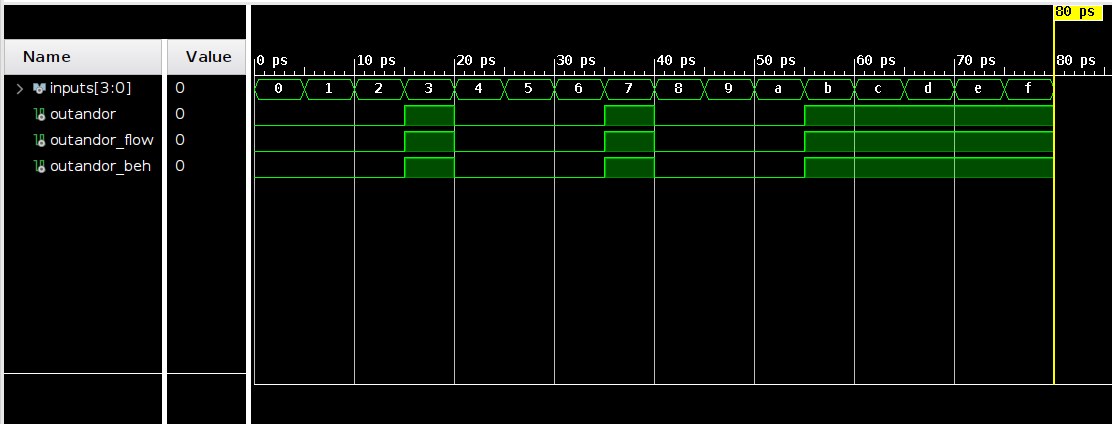
\includegraphics[scale=0.25]{images/simulation_no_delay.png}
    \caption{AND2OR simulation without any delays applied}
    \label{fig:simulation_no_delay}
\end{figure}

As can be seen in figure \ref{fig:simulation_no_delay}, the $outandor$, $outandor \_ flow$ and $outandor \_ beh$ each have identical output values which correspond with the truth values specified within table \ref{tab:truth_table}. This indicates that the entire system is working as expected. However, it has not fully proven the test bed's ability to detect simulation errors. 

For this reason, a secondary test was conducted in which the error checking was intentionally changed. This test scenario was designed such that the test bed expected an output of 0 for $outandor$ when an input of $a=1$ and $b=1$ was provided. Obviously, this would not happen since $a \cap b=1$. In this situation, a system error was to be thrown which would display within Vivado's console. The successful outputs of this altered test can be found within figure \ref{fig:errors}.

\begin{figure}[H]
    \centering
    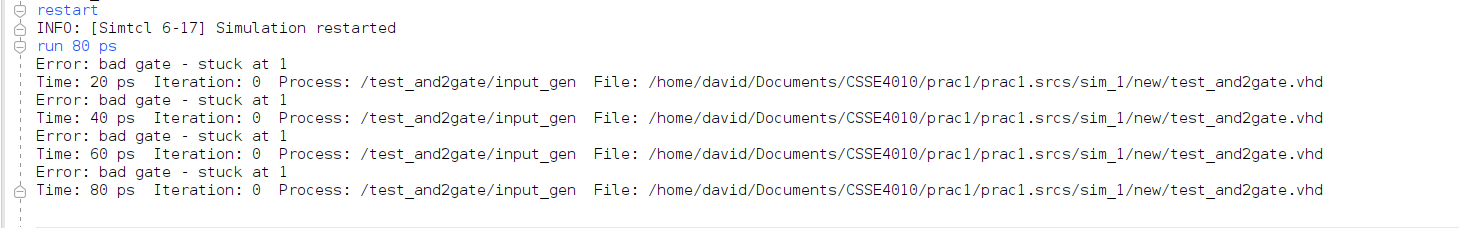
\includegraphics[scale=0.25]{images/error.png}
    \caption{Console outputs for an intentional error for inputs A and B}
    \label{fig:errors}
\end{figure}

At this point, it has been proven that both the test bed and the AND2OR file are functioning as expected. The final simulation required the integration of a propagation delay into the system, to emulate the delays experienced due to physical components in real life. To achieve this, a propagation delay was applied to the output $outandor \_ beh$, which could be seen to have a staggered and delayed output compared to the rest of the system. This could be seen within figure \ref{fig:delay}

\begin{figure}[H]
    \centering
    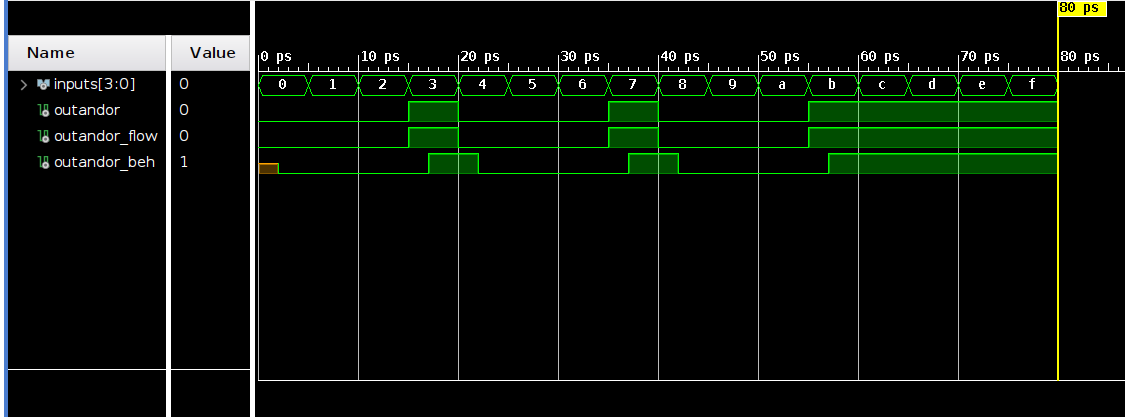
\includegraphics[scale=0.25]{images/delays.png}
    \caption{Simulated output for AND2OR with delay}
    \label{fig:delay}
\end{figure}

In total, the design was functionally correct. It displayed the correct outputs, had the correct error checking and was able to properly integrate delays.

\section{Synthesis and Implementation Results}

Upon completing the simulation, it was now necessary to run a synthesis model. This provides a generalised model upload model of the program, which can be further refined by running an implementation. The results of the model's synthesis can be found in figure \ref{fig:synthesis}

\begin{figure}[H]
    \centering
    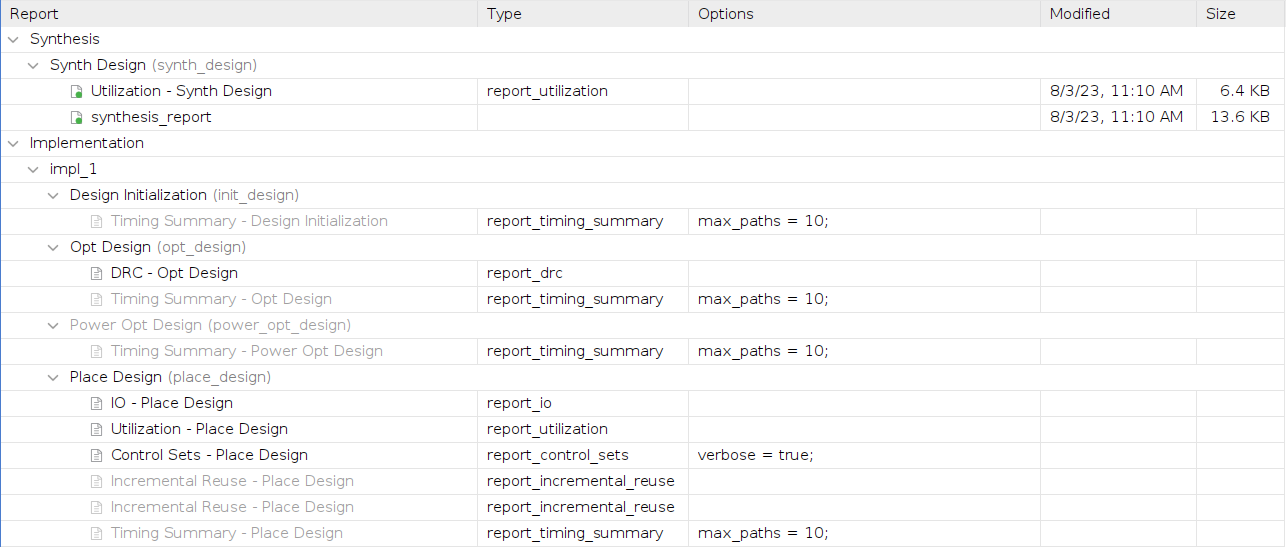
\includegraphics[scale=0.25]{images/synthesis_results_1.png}
\end{figure}
\begin{figure}[H]
    \centering
    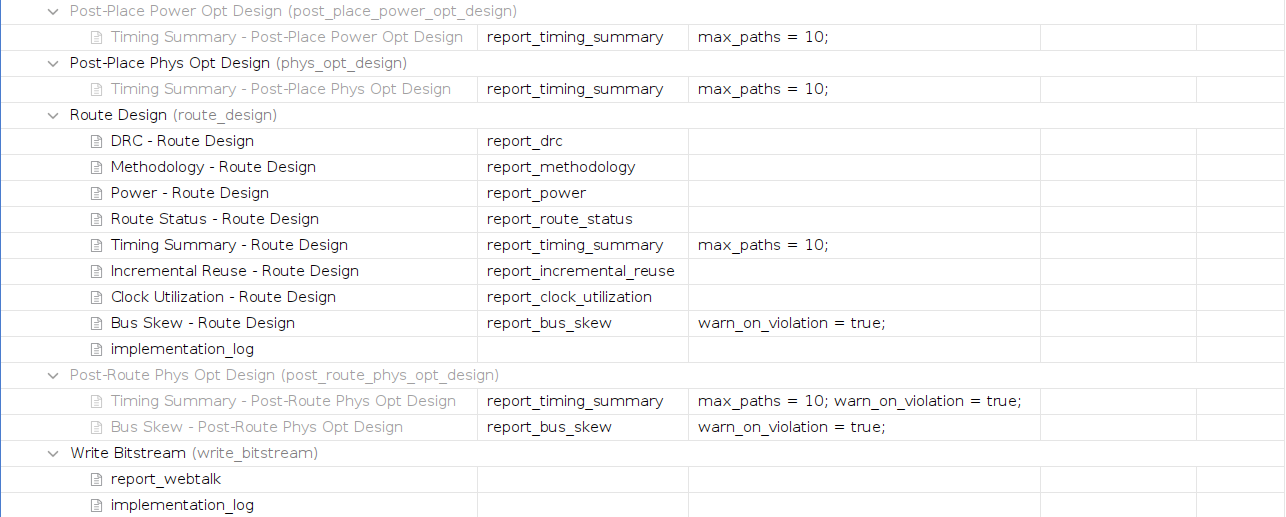
\includegraphics[scale=0.25]{images/synthesis_results_2.png}
    \caption{Results of synthesis}
    \label{fig:synthesis}
\end{figure}

Furthermore, the utilisation of the system for running this design can be found in figure \ref{fig:utilisation}. Note that only a fractional percentage 3$\%$ of the board I/O was utilised, as well as one of the 63400 available lookup tables. This could be confirmed upon close analysis into the implemenation's architecture (But that goes far beyond the scope of this assignment. That's a deep, dark world in there).

\begin{figure}[H]
    \centering
    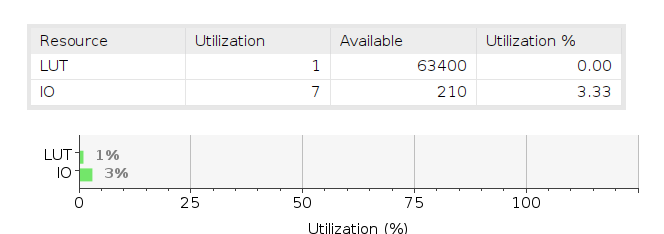
\includegraphics[scale=0.5]{images/utilization.png}
    \caption{Utilisation report for AND2OR}
    \label{fig:utilisation}
\end{figure}


\section{Discussion and Conclusion}

In conclusion, it can be seen that the system functions fully as expected. The AND2OR file is able to correctly create the the system shown in figure \ref{fig:cct}, which maps to the outputs shown in table \ref{tab:truth_table}. Error checking has been verified, and the system was able to fully integrate delays. Lastly, the model was able to synthesize and provide outputs to the implementation process as described within its corresponding section.

In total, the entire system works, and there is no need for improvement.

\section{Appendices}

\begin{figure}[H]
    \centering
    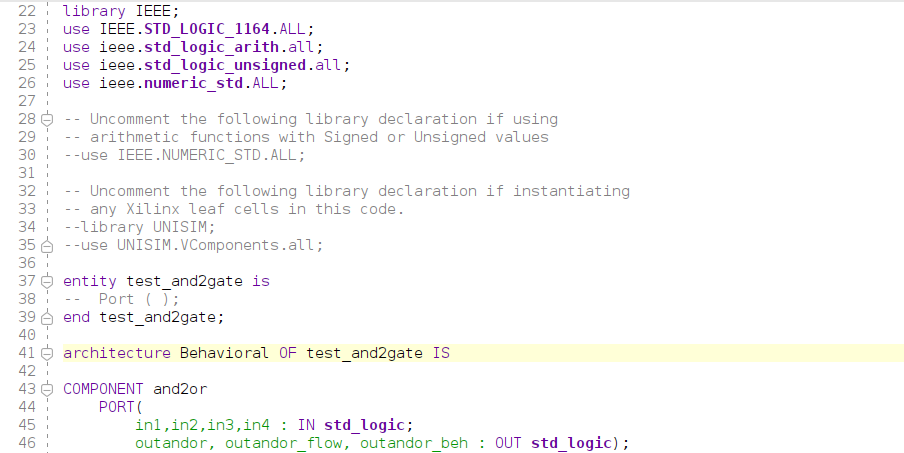
\includegraphics[scale=0.25]{images/code 1.png}
\end{figure}
\begin{figure}[H]
    \centering
    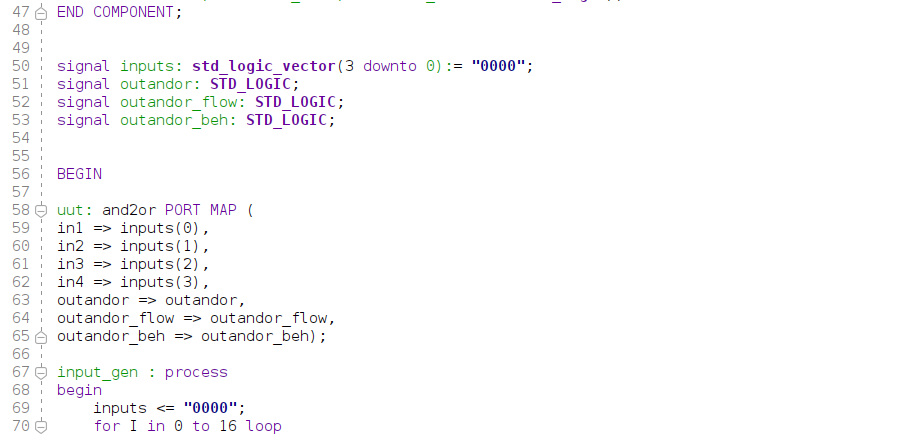
\includegraphics[scale=0.25]{images/code 2.png}
\end{figure}
\begin{figure}[H]
    \centering
    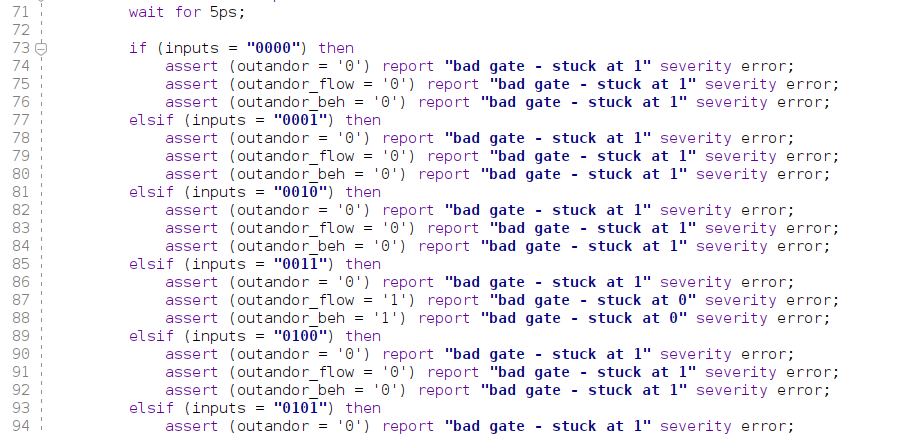
\includegraphics[scale=0.25]{images/code 3.png}
\end{figure}
\begin{figure}[H]
    \centering
    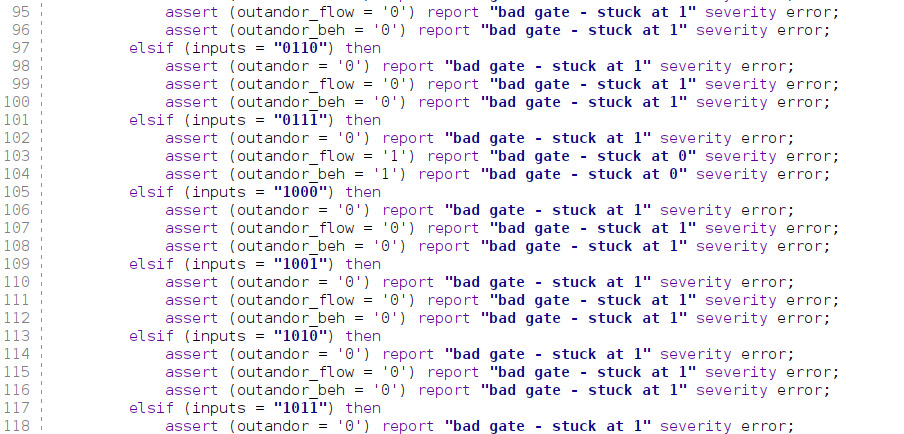
\includegraphics[scale=0.25]{images/code 4.png}
\end{figure}
\begin{figure}[H]
    \centering
    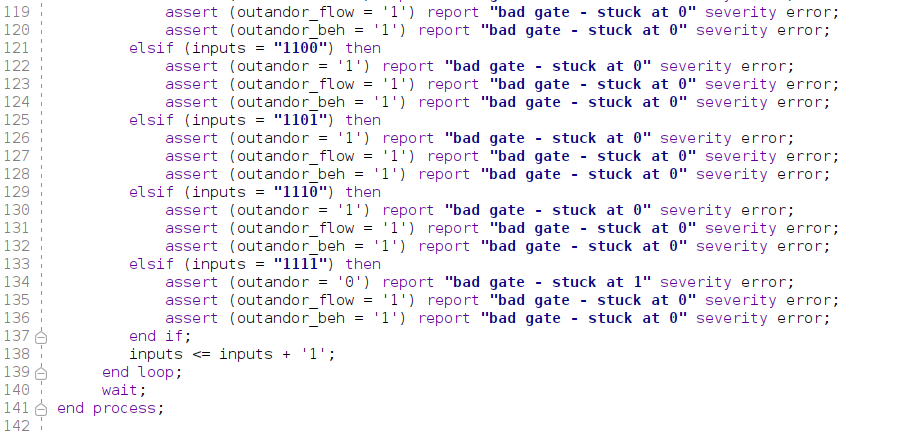
\includegraphics[scale=0.25]{images/code 5.png}
\end{figure}



Do you remember in 2019 how bushfires ravaged 17 million hectares of Australian soil;  close to 50 times the landmass of Germany? In that time, 33 lives, 3'094 houses and one billion animals were consumed consumed in those flames. Ideally, prevention is the best cure, but due to the time and cost associated with assessing potential bushfire threats, National Park rangers and the Royal Fire Brigade lack the propensity to address every hazard before it's too late. If there was a way to assist them with the on-the-ground coverage of these threats, it would save over 1.5 billion dollars annually, as well as ensure the safety of our country. 

\end{document}
